% !TeX TS-program = xelatex

\documentclass[aspectratio=169]{beamer}

\usepackage{xltxtra}
\usepackage[main=russian,english]{babel}
\defaultfontfeatures{Mapping=tex-text}
\usepackage{listings}
\usepackage[backend=biber,bibstyle=numeric,citestyle=numeric-comp,sorting=none,defernumbers=true,date=long]{biblatex}
\addbibresource{dumpparsing.bib}

\makeatletter
\let\old@lstKV@SwitchCases\lstKV@SwitchCases
\def\lstKV@SwitchCases#1#2#3{}
\makeatother
\usepackage{lstlinebgrd}
\makeatletter
\let\lstKV@SwitchCases\old@lstKV@SwitchCases

\lst@Key{numbers}{none}{%
    \def\lst@PlaceNumber{\lst@linebgrd}%
    \lstKV@SwitchCases{#1}%
    {none:\\%
     left:\def\lst@PlaceNumber{\llap{\normalfont
                \lst@numberstyle{\thelstnumber}\kern\lst@numbersep}\lst@linebgrd}\\%
     right:\def\lst@PlaceNumber{\rlap{\normalfont
                \kern\linewidth \kern\lst@numbersep
                \lst@numberstyle{\thelstnumber}}\lst@linebgrd}%
    }{\PackageError{Listings}{Numbers #1 unknown}\@ehc}}
\makeatother

\setmainfont{Arial}
%\setromanfont{Times New Roman}
%\setsansfont{Arial}
%\setmonofont{Courier New}

\title{Разбор и сравнение данных в большом XML на маленькой VDS}
\author{Филипп Кулин (Эшер II)}
\date{08 февраля 2020 года, Казань}

\usetheme{gck022020}

\setbeamercolor{itemize item}{fg=text}
\setbeamercolor{itemize subitem}{fg=text}
\setbeamercolor{alerted text}{fg=text}
\setbeamertemplate{itemize items}{\textbullet}
\setbeamerfont*{itemize/enumerate subbody}{parent=itemize/enumerate body}
\setbeamerfont*{itemize/enumerate subsubbody}{parent=itemize/enumerate subbody}
\setbeamerfont{alerted text}{series=\bfseries}

\definecolor{acmebg}{HTML}{FFFFEF}
\definecolor{acmeh}{HTML}{EFFFFF}
\definecolor{acmec}{HTML}{8C8ACE}
\definecolor{acmel}{HTML}{52AAAD}
\definecolor{acmel1}{HTML}{EFEF9C}
\definecolor{acmel2}{HTML}{9CEFEF}
\lstset{
        columns=flexible,
        keepspaces=true,
        showstringspaces=false,
        showtabs=false,
        tabsize=4,
        frame=single,
        basicstyle=\fontsize{10pt}{12}\bf\ttfamily\color{black},
        %basicstyle=\bf\tiny\ttfamily\color{black},
        backgroundcolor=\color{acmebg},
        commentstyle=\color{black},
        keywordstyle=\color{black},
        stringstyle=\color{red},
        rulecolor=\color{acmel},
        framerule=1pt,
        inputencoding=utf8,
        escapeinside={\%*}{*)}
        %moredelim=**[is][\only<+>{\colorbox{acmel1}{#1}}]{@}{@},
}

\setbeamerfont{bibliography item}{size*={8pt}{1}}
%\setbeamerfont{bibliography entry author}{size*={8pt}{1}}
%\setbeamerfont{bibliography entry title}{size*={8pt}{1}}
%\setbeamerfont{bibliography entry location}{size*={8pt}{1}}
%\setbeamerfont{bibliography entry note}{size*={8pt}{1}}
%\setbeamercolor{bibliography entry author}{fg=text, bg=}
%\setbeamercolor{bibliography entry title}{fg=text, bg=}
%\setbeamercolor{bibliography entry location}{fg=blue, bg=}
%\setbeamercolor{bibliography entry note}{fg=text, bg=}
%\setbeamertemplate{bibliography entry article}{}
%\setbeamertemplate{bibliography entry title}{}
%\setbeamertemplate{bibliography entry location}{}
%\setbeamertemplate{bibliography entry note}{}
%\setbeamertemplate{bibliography item}[text]

% for biblatex
\setbeamertemplate{bibliography item}{\insertbiblabel}
\renewcommand*{\bibfont}{\fontsize{8}{1}\selectfont}
\DeclareFieldFormat{url}{\color{blue}\url{#1}}


\newcommand{\clbox}[2]{%
  \hspace*{-\fboxsep}\colorbox{#1}{#2}\hspace*{-\fboxsep}%
}

\makeatletter
%%%%%%%%%%%%%%%%%%%%%%%%%%%%%%%%%%%%%%%%%%%%%%%%%%%%%%%%%%%%%%%%%%%%%%%%%%%%%%
%
% \btIfInRange{number}{range list}{TRUE}{FALSE}
%
% Test in int number <number> is element of a (comma separated) list of ranges
% (such as: {1,3-5,7,10-12,14}) and processes <TRUE> or <FALSE> respectively

\newcount\bt@rangea
\newcount\bt@rangeb

\newcommand\btIfInRange[2]{%
    \global\let\bt@inrange\@secondoftwo%
    \edef\bt@rangelist{#2}%
    \foreach \range in \bt@rangelist {%
        \afterassignment\bt@getrangeb%
        \bt@rangea=0\range\relax%
        \pgfmathtruncatemacro\result{ ( #1 >= \bt@rangea) && (#1 <= \bt@rangeb) }%
        \ifnum\result=1\relax%
            \breakforeach%
            \global\let\bt@inrange\@firstoftwo%
        \fi%
    }%
    \bt@inrange%
}
\newcommand\bt@getrangeb{%
    \@ifnextchar\relax%
        {\bt@rangeb=\bt@rangea}%
        {\@getrangeb}%
}
\def\@getrangeb-#1\relax{%
    \ifx\relax#1\relax%
        \bt@rangeb=100000%   \maxdimen is too large for pgfmath
    \else%
        \bt@rangeb=#1\relax%
    \fi%
}

%%%%%%%%%%%%%%%%%%%%%%%%%%%%%%%%%%%%%%%%%%%%%%%%%%%%%%%%%%%%%%%%%%%%%%%%%%%%%%
%
% \btLstHL<overlay spec>{range list}
%
% TODO BUG: \btLstHL commands can not yet be accumulated if more than one overlay spec match.
% 
\newcommand<>{\btLstHL}[1]{%
\only#2{\btIfInRange{\value{lstnumber}}{#1}{\color{acmel1}\def\lst@linebgrdcmd{\color@block}}{\def\lst@linebgrdcmd####1####2####3{}}}%
}%
\makeatother

\begin{document}

\begin{frame}
\titlepage
\end{frame}

\begin{frame}{Откиньтесь на спинку кресла}
        \begin{itemize}
                \item Эта презентация сделана с помощью \LaTeX \supercite{habrlatex}
                \item Избежать большого количества кода не удалось
                \item Материал основан на работающем сервисе \supercite{u2ckdump}
                \item Значительная часть кода написана сообществом
        \end{itemize}
\end{frame}

\begin{frame}{Задача}
        \textbf{Что надо было сделать}
        \begin{itemize}
                \item<1-> Разобрать XML-файл в 160Mb и положить в базу
                \item<1-> Обновлять базу по новым XML-файлам
                \item<1-> Предоставить интерфейс для доступа к базе
        \end{itemize}
        \onslide<2-> \textbf{Условия}
        \begin{itemize}
                \item<2-> Скорость разбора — единицы минут
                \item<2-> Недорогой виртуальный сервер
                \item<2-> Приоритет стандартных решений
        \end{itemize}
\end{frame}

\begin{frame}{Интересная задача}
        \begin{itemize}
                \item \textbf{Никаких инноваций и "rocket science"}
                \item Навязанные условия
                \item Чувствительность к работе памяти
                \item Чувствительность к ресурсам
                \item Хрестоматийные решения
        \end{itemize}
\end{frame}

\begin{frame}{Гадание}
        \begin{itemize}
                \item<1-> Не всегда очевидны «тонкие» места
                \item<1-> Абстракции — «тихие омуты»
                \item<2-> Тесты, бенчмарки, профилирование
        \end{itemize}
\end{frame}

\begin{frame}{Архитектура}
        \begin{itemize}
                \item База данных
                \item Индексы по значениям для поиска
                \item Функционал наполнения базы из исходных данных
                \item Функционал обновления данных
                \item Функционал поиска данных
        \end{itemize}
\end{frame}

\begin{frame}[fragile,label=reg]{Формат исходных данных. XML}
        \begin{itemize}
                \item<1-> 250 тысяч элементов \texttt{content}
                \item<1-> Размер каждого от сотни байт до \textbf{6}MB
                \item<1-> Общий размер данных свыше \textbf{150}MB
                \item<2-> XML в кодировке CP1251
        \end{itemize}
        \begin{lstlisting}[linewidth=\textwidth,xleftmargin=0.04\textwidth,basicstyle=\fontsize{14pt}{14}\bf\ttfamily\color{black},linebackgroundcolor={\btLstHL<2>{1}}]
<?xml version="1.0" encoding="windows-1251"?>
<reg:register ...>
        <content id="656" ...> ... </content>
        ...
        <content id="2062369" ...> ... </content>
</reg:register>\end{lstlisting}
\end{frame}

\begin{frame}[fragile,label=scheme]{Элемент Content}
        \begin{lstlisting}[linewidth=0.8\textwidth,xleftmargin=0.04\textwidth]
<content id="680741"...>
        <decision .../>
        <domain><![CDATA[example.com]]></domain>
        <url><![CDATA[https://example.com/smt]]></url>
        ...
        <ip>10.0.0.1</ip>
        ...
        <ipv6>fc00::beef</ipv6>
        ...
        <ipSubnet>10.1.0.0/16</ipSubnet>
        ...
        <ipSubnet6>fd00::/48</ipSubnet6>
        ...
</content>\end{lstlisting}
        \begin{itemize}
                \item IP-адреса могут быть поштучно тысячами
        \end{itemize}
\end{frame}

\begin{frame}[fragile]{Потоковый разбор XML}
        \begin{itemize}
                \item<2-> Создаем декодер
                \item<3-> Не забываем про кодировку
                \item<4-> Ловим каждый элемент
        \end{itemize}
        \begin{lstlisting}[linewidth=0.75\textwidth,xleftmargin=0.04\textwidth,linebackgroundcolor={\btLstHL<2>{3}%
                                                \btLstHL<3>{4}%
                                                \btLstHL<4>{6}%
                                                }]
import "encoding/xml"
...
decoder := xml.NewDecoder(dumpFile)
decoder.CharsetReader = charset.NewReaderLabel
for {
        t, err := decoder.Token()
        ...
        switch _e := t.(type) {
        case xml.StartElement:
                switch _e.Name.Local {
                case "content":
...\end{lstlisting}
\end{frame}

\begin{frame}{Выбор формы хранения данных}
        \begin{itemize}
                \item<1-> Время разбора XML — 10-200 секунд
                \item<2-> База нужна только для хранения
                \item<3-> bbolt — заполнение час+
                \item<4-> map + скорость разбора = \textbf{победа}
        \end{itemize}
\end{frame}

\againframe{reg}

\begin{frame}[fragile]{Формат хранения данных}
        \begin{itemize}
                \item<1-> Каждый \texttt{content} имеет уникальный числовой \texttt{id}
                \item<1-> \texttt{id} очень разреженные
                \item<2-> Решение: \texttt{map[int]*TContent}\\
                        \texttt{TContent} — структура для \texttt{DecodeElement()}
                        \begin{lstlisting}[linewidth=0.9\textwidth,basicstyle=\fontsize{14pt}{14}\bf\ttfamily\color{black},linebackgroundcolor={\btLstHL<2>{2}}]
case "content":
        err := decoder.DecodeElement(&v, &_e)\end{lstlisting}
         \end{itemize}
\end{frame}

\begin{frame}{Хранение данных. Грабли}
        \begin{itemize}
                \item<1-> Уменьшаем аллокации
                \item<2-> Улучшательство: \texttt{map[int]TContent}
                \item<3-> \textbf{Боль} \only<4->{программы ощущалась физически...}
                \item<4-> Расширение карты — очень дорогая операция
                \item<4-> Всё-таки \texttt{map[int]*TContent}
        \end{itemize}
\end{frame}

\begin{frame}[fragile]{Хранение данных. Оптимизация}
        \begin{itemize}
                \item<1-> Часть элементов имеет аттрибут \texttt{ts}:
                        \begin{lstlisting}[linewidth=0.75\textwidth,basicstyle=\fontsize{14pt}{14}\bf\ttfamily\color{black}]
ts="2020-02-06T19:54:00+03:00"\end{lstlisting}
                \item<1-> IPv4-адреса представлены элементом IP:
                        \begin{lstlisting}[linewidth=0.75\textwidth,basicstyle=\fontsize{14pt}{14}\bf\ttfamily\color{black}]
<ip ts="2020-02-06T19:54:00+03:00">
        10.0.0.1
</ip>\end{lstlisting}
                \item<2-> Две строки против двух целых чисел
                \item<2-> Миллионы структур c IPv4-адресами
        \end{itemize}
\end{frame}

\begin{frame}[fragile]{Оптимизация конвертации данных}
	\begin{itemize}
		\item<1-> Преобразование стандартными средствами 
			\begin{lstlisting}
ip := net.ParseIP(s)
intIp =: binary.BigEndian.Uint32(ip[12:16])\end{lstlisting}
		\item<2-> Пишем менее универсально, но без аллокаций
		\item<3-> Сравниваем
			\begin{lstlisting}
Benchmark_Standart-4  4295910  268   ns/op  48 B/op  3 allocs/op
Benchmark_Custom-4   18941194   60.8 ns/op   0 B/op  0 allocs/op\end{lstlisting}
	\end{itemize}
\end{frame}

\begin{frame}[fragile,label=unmar]{Более детальное преобразование}
        \begin{itemize}
                \item Наполняем \texttt{TContent} «вручную»
                \item<2-> Значительное уменьшение потребления памяти
        \end{itemize}
        \begin{lstlisting}[linewidth=\textwidth,xleftmargin=0.04\textwidth,linebackgroundcolor={\btLstHL<1>{2}%
                                                \btLstHL<2>{3,5,11}%
                                                }]
case "content":
%*\only<2>{\% }*)err := decoder.DecodeElement(&v, &_e)
%*\only<1>{\% }*)err := UnmarshalContent(tempBuf, &v)                        
...
func UnmarshalContent(b []byte, v *TContent) error {
    buf := bytes.NewReader(b)
    decoder := xml.NewDecoder(buf)
    ...
    case elementIp:
        ip := TXMLIp{}
        if err := decoder.DecodeElement(&ip, &element); err != nil {\end{lstlisting}
\end{frame}

\begin{frame}{Хранение данных. Индексы}
        \begin{itemize}
                \item Самая простая и скучная часть
                \item map нужных данных
                \item Значения — массивы \texttt{id} элементов \texttt{content}
        \end{itemize}
\end{frame}

\begin{frame}{Обновление данных}
        \begin{itemize}
                \item<1-> Упрощаем до сравнения \texttt{content} целиком
                \item<2-> Считаем контрольные суммы
        \end{itemize}
\end{frame}

\begin{frame}{Контрольные суммы}
        \begin{itemize}
                \item<1-> Считал SHA256
                \item<2-> Профилирование показало, что выбор неудачный
                \item<3-> Выбрал на 64-bit FNV-1
                \begin{itemize}
                        \item<4-> Проверил, заглянув «под капот»
                \end{itemize}
        \end{itemize}
\end{frame}

\begin{frame}{Как считаем контрольные суммы}
        \begin{itemize}
                \item<1-> Преобразование \texttt{TContent} обратно в XML
                        \begin{itemize}
                                \item<2-> Требует двойного преобразования \textbf{каждого} элемента
                        \end{itemize}
                \item<3-> Использование \texttt{io.TeeReader}
                        \begin{itemize}
                                \item<4-> Декодируем только изменившиеся элементы \texttt{content}
                        \end{itemize}
        \end{itemize}
\end{frame}

\begin{frame}[fragile]{TeeReader и Decoder. Грабли №1}
        \begin{lstlisting}[linewidth=0.95\textwidth,basicstyle=\fontsize{14pt}{14}\bf\ttfamily\color{black},linebackgroundcolor={\btLstHL{1,5}}]
tr := io.TeeReader(dumpFile, &buffer)
decoder := xml.NewDecoder(tr)
decoder.CharsetReader = charset.NewReaderLabel
for {
        tokenStartOffset := decoder.InputOffset()\end{lstlisting}
        \begin{itemize}
                \item<2-> ... не работает, данные не синхронны
                \item<3-> XML декодер «шагает» по UTF-8 строке
                \item<3-> контрольные суммы «шагают» по CP1251 строке
        \end{itemize}
\end{frame}

\begin{frame}[fragile]{TeeReader и Decoder. Грабли №2}
        \begin{lstlisting}[linewidth=0.95\textwidth,basicstyle=\fontsize{12pt}{12}\bf\ttfamily\color{black},linebackgroundcolor={\btLstHL{5}}]
decoder := xml.NewDecoder(dumpFile)
decoder.CharsetReader = 
        func(l string, i io.Reader) (io.Reader, error) {
        r, err := charset.NewReaderLabel(l, i)
        return io.TeeReader(r, &buffer), nil
}
for {
        tokenStartOffset := decoder.InputOffset()\end{lstlisting}
        \begin{itemize}
                \item<2-> ... не работает, данные не синхронны
                \item<3-> XML декодер «перепрыгивает» через заголовок 
                \item<3-> контрольные суммы не «перепрыгивают»
        \end{itemize}
\end{frame}

\begin{frame}[fragile]{TeeReader и Decoder}
        Заработало!
        \begin{lstlisting}[linewidth=0.95\textwidth,basicstyle=\fontsize{12pt}{12}\bf\ttfamily\color{black},linebackgroundcolor={\btLstHL{5}}]
decoder := xml.NewDecoder(dumpFile)
decoder.CharsetReader = 
        func(l string, i io.Reader) (io.Reader, error) {
        r, err := charset.NewReaderLabel(l, i)
        offsetCorrection = decoder.InputOffset()
        return io.TeeReader(r, &buffer), nil
}
for {
        tokenStartOffset := decoder.InputOffset() -
                offsetCorrection\end{lstlisting}
\end{frame}

\begin{frame}{Отличное наглядное упражнение}
        \begin{itemize}
                \item Ридеры/райтеры — go-way
                \item I/O через буфер тянется ещё с 90-ых
                \item Ридеры/райтеры на интерфейсах — новое в go
                \item У новичков затруднено понимание этой абстракции
                \item Хороший пример использования «замыкания»
                \item Разобранная задача — отличное упражнение
        \end{itemize}
\end{frame}

\begin{frame}{Подключаем gRPC}
        \begin{itemize}
                \item<1-> Универсальное простое рабочее решение
                \item<2-> Данные хранить сразу в формате gRPC
                \begin{itemize}
                        \item<3-> gRPC пытается всё хранить ссылками
                        \item<4-> Несовместимо с нашей борьбой со ссылками
                \end{itemize}
        \end{itemize}
\end{frame}

\begin{frame}{Делаем промежуточный тип}
        \begin{itemize}
                \item<1-> Из XML преобразуем в \texttt{TContent}
                \item<2-> \texttt{TContent} пакуем в json
                \item<3-> Новый тип \texttt{TMinContent} содержит:
                \begin{itemize}
                        \item<3-> метаданные
                        \item<3-> данные для сравнения (и индекса)
                        \item<3-> контрольную сумму для сравнения
                        \item<3-> Полные данные \texttt{TContent} в виде json
                \end{itemize}
                \item<4-> В базу кладем \texttt{TMinContent}
                \item<5-> Увеличен общий объём данных из-за дублирования
        \end{itemize}
\end{frame}

\begin{frame}{Данные gRPC}
        \begin{itemize}
                \item<1-> Массив «сообщений». «Сообщение» содержит:
                        \begin{itemize}
                                \item<1-> метаданные
                                \item<1-> полные данные в виде json-строки с \texttt{TContent}
                        \end{itemize}
                \item<2-> Буфер под отдаваемые данные минимален
                \item<3-> \textit{Можно написать свою реализацию gRPC}
        \end{itemize}
\end{frame}

\begin{frame}{}
        \center {\Huge Что ещё можно «подкрутить»?}
\end{frame}

% Кусок про память и настройки рантайма
\begin{frame}{Использование памяти}
        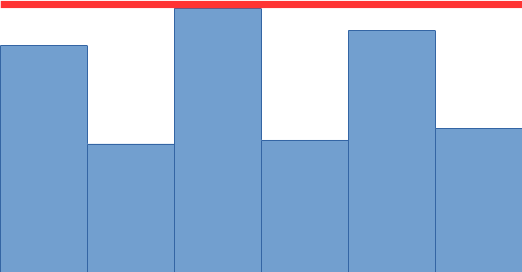
\includegraphics[width=0.75\textwidth]{mem.png}\\
        Нас интересует только верхняя граница
\end{frame}

\begin{frame}[fragile]{Настройки рантайма}
        \begin{itemize}
                \item<1-> Управление сборщиком мусора
                \begin{lstlisting}[linewidth=0.75\textwidth,basicstyle=\fontsize{14pt}{14}\bf\ttfamily\color{black}]
% GOGC=50 /bin/myapp\end{lstlisting}
                \begin{itemize}
                        \item<2-> Малоэффективно, «подтормаживает»
                \end{itemize}
                \item<3-> Возврат памяти системе
                \begin{lstlisting}[linewidth=0.75\textwidth,basicstyle=\fontsize{14pt}{14}\bf\ttfamily\color{black}]
% GODEBUG=madvdontneed=1 /bin/myapp\end{lstlisting}
                \begin{itemize}
                        \item<4-> Малоэффективно в пике, «тормозит»
                \end{itemize}
        \end{itemize}
        \onslide<5-> \textbf{Чем хуже код — тем больше негативный эффект}
\end{frame}

\begin{frame}{Итог}
        \begin{itemize}
                \item Данные в map в памяти
                \item map для индексов
                \item Хранения на диске нет
                \item Потоковый разбор XML с TeeReader
                \item Оптимизация форматов данных
                \item Сравнение через контрольные суммы
                \item Вспомогательный тип для хранения данных
        \end{itemize}
\end{frame}

\begin{frame}{Вопросы}
        \center Избави, Боже, нас от ярости норманнов \\и «интересных задач»
        \vskip2cm
        \center{schors@gmail.com}
\end{frame}

\nocite{*}
\setbeamertemplate{frametitle continuation}{}

\begin{frame}[t]{Ссылки}
\printbibliography[notkeyword={en}]
\end{frame}

\end{document}


